\section{Resultados e Discussão}
\label{sec:resultados}

Esta seção consolida as métricas obtidas nos testes de carga (k6) e no ensaio assíncrono com Cloud Tasks. As análises seguem os SLIs definidos na metodologia: latência P95, taxa de erro e comportamento das filas sob acúmulo de tarefas. O objetivo é verificar a aderência da arquitetura aos SLOs estabelecidos e compreender os pontos de saturação observados.

\begin{table}[ht]
    \centering
    \caption{Resumo dos cenários de carga e conformidade com os SLOs}
    \label{tab:resultados_k6}
    \begin{tabular}{lcccc}
        \toprule
        Cenário & Latência P95 & Throughput médio & Throughput pico & Taxa de erro \\
        \midrule
        Leitura intensiva & 158~ms & 470 req/s & 970 req/s & 0{,}00\% \\
        Mistura leitura/escrita & 658~ms & 226 req/s & 450 req/s & 0{,}00\% \\
        \bottomrule
    \end{tabular}
\end{table}

Os valores de \textit{throughput} foram extraídos diretamente dos dashboards do Cloud Run, refletindo o número real de requisições por segundo atendidas por todas as instâncias durante cada estágio do teste. Assim, VUs e req/s representam perspectivas complementares do mesmo nível de pressão sobre o sistema.

\subsection{Cenário de Leitura Intensiva}

O cenário de leitura mobilizou 1.000 usuários virtuais por 17 minutos, sustentando em média 470 requisições por segundo e alcançando um pico próximo a 970 req/s no trecho final ($900\rightarrow 1.000$ VUs). A latência P95 permaneceu em 158~ms (Tabela~\ref{tab:resultados_k6}), substancialmente abaixo do SLO de 300~ms, e nenhuma requisição apresentou erro. Esses resultados confirmam que o caminho otimizado de leitura — CDN, API em Cloud Run, Redis como cache e consultas eficientes no PostgreSQL — suporta picos significativos de tráfego sem degradação perceptível.

O Cloud Monitoring registrou o escalonamento completo das 10 instâncias de Cloud Run, atingindo CPU média de 72\% e uso de memória em torno de 31\%. Ou seja, a cota máxima de CPU foi totalmente utilizada, mas sem sinais de exaustão ou sobrecarga que pudessem comprometer as latências observadas.

\begin{figure}[ht]
    \centering
    \includegraphics[width=0.95\linewidth]{figures/fig-read-pxx.png}
    \caption{Latências P50/P95/P99 por carga (VUs) no cenário de leitura. A linha tracejada indica o SLO de 300~ms, não violado durante o teste.}
    \label{fig:latencia-leitura}
\end{figure}

\subsection{Cenário Misto (Leitura/Escrita)}

O cenário misto utilizou provisionamento automático de contas e tokens por VU, eliminando o gargalo artificial presente em versões anteriores do teste.
Com 650 usuários alternando entre 65\% de leituras e 35\% de escritas durante 21 minutos, o sistema sustentou 226 requisições por segundo ($\approx 283$ mil iterações) sem erros e manteve o SLO de 300~ms até aproximadamente 450 RPS.
A violação sistemática do SLO ocorre por volta de 539 VUs, ponto a partir do qual o Cloud Run volta a atingir o limite de 10 instâncias.

Nos estágios acima de 550 VUs, o P95 consolidado do ensaio alcançou 658~ms, enquanto o p99 atingiu 2,67~s. A origem da degradação é clara: o caminho de escrita demanda mais CPU por requisição (validações, transações ACID e invalidação de cache), reduzindo a capacidade de requisições por instância quando o limite de contêineres é atingido. As métricas do Cloud SQL mostraram estabilidade, indicando que o banco relacional não foi o gargalo primário nesse experimento.

\begin{figure}[ht]
    \centering
    \includegraphics[width=0.95\linewidth]{figures/fig-mixed-pxx.png}
    \caption{Latências P50/P95/P99 por carga (VUs) no cenário misto. A faixa tracejada marca o SLO de 300~ms; etapas acima de 539~VUs apresentam violações persistentes.}
    \label{fig:latencia-mix}
\end{figure}

A Figura~\ref{fig:comparacao} ilustra o distanciamento entre os comportamentos das duas cargas. Enquanto o cenário de leitura mantém o P95 abaixo de 200~ms mesmo no pico de 1.000 VUs, o cenário misto diverge abruptamente após 500 VUs. Esse comportamento é consistente com modelos teóricos de sistemas transacionais \cite{kleppmann_ddia_2017}, segundo os quais rotas de escrita têm custo marginal crescente e menor paralelização efetiva, sobretudo em sistemas baseados em contêineres com cotas rígidas de CPU.

\begin{figure}[ht]
    \centering
    \includegraphics[width=0.95\linewidth]{figures/fig-compare-read-vs-mixed.png}
    \caption{Comparação entre os P95 dos cenários de leitura e misto. A leitura permanece estável; a escrita viola o SLO acima de 539~VUs.}
    \label{fig:comparacao}
\end{figure}

Os resultados reforçam que, antes de adotar mecanismos mais complexos (particionamento, réplicas dedicadas ou CQRS físico), a arquitetura pode obter ganhos expressivos liberando o limite de instâncias HTTP no Cloud Run ou reduzindo o custo computacional por escrita.

\subsection{Processamento Assíncrono com Cloud Tasks}

O ensaio assíncrono publicou 51{,}58 mil tarefas em lote e monitorou a drenagem entre 01:08 e 01:18 ($\approx 10$ minutos). Isso corresponde a aproximadamente 86 tarefas/segundo processadas em média, com variação alinhada ao número de instâncias de worker ativadas dinamicamente. O Cloud Run escalou horizontalmente enquanto havia backlog, reduzindo o número de instâncias assim que o volume de tarefas diminuiu.

Nenhuma entrega foi perdida ou duplicada. A latência ponta-a-ponta permaneceu estável porque:

\begin{itemize}
    \item o Cloud Tasks opera em modo \textit{push}, eliminando \textit{polling};
    \item o Redis atuou somente como \textit{backplane} de eventos e não participou do pipeline crítico;
    \item cada worker pôde operar de forma idempotente e independente.
\end{itemize}

Esse comportamento demonstra elasticidade eficiente: a infraestrutura permanece mínima em períodos ociosos e escala agressivamente apenas durante janelas de pico, alinhando custo e demanda sem intervenção manual.

\begin{figure}[ht]
    \centering
    \includegraphics[width=0.95\linewidth]{figures/fig-queue-drain.png}
    \caption{Taxa de processamento das filas (tarefas/min) e janela de drenagem entre 01:08 e 01:18 no ensaio com Cloud Tasks.}
    \label{fig:filas}
\end{figure}

\subsection{Síntese e Discussão Integrada}

Os resultados demonstram que:

\begin{itemize}
    \item \textbf{O caminho de leitura é altamente escalável}, atendendo 1.000 VUs com folga e sem violar SLOs.
    \item \textbf{O caminho de escrita é limitado pela cota de CPU do Cloud Run}, não pelo banco.
    \item \textbf{O pipeline assíncrono é elástico e confiável}, drenando grandes volumes sem perda de tarefas.
    \item \textbf{A arquitetura é adequada para workloads dominados por leitura}, mas exige ajustes para workloads de escrita concorrente.
\end{itemize}

Esses achados orientam recomendações para escalabilidade futura, incluindo aumento das cotas de instâncias, separação de serviços de escrita, redução do custo computacional das rotas críticas e, eventualmente, adoção de padrões arquiteturais como CQRS físico ou particionamento de dados.

\subsection{Análise de Custos Operacionais e Trade-offs de Elasticidade}
\label{sec:analise_custos}

Embora o foco principal deste trabalho esteja no desempenho e na validação dos SLOs, a análise de custos é essencial para avaliar a viabilidade da arquitetura. Os serviços utilizados — especialmente o Cloud Run — possuem modelos de cobrança distintos dos ambientes tradicionais baseados em máquinas virtuais (Compute Engine), o que altera significativamente a dinâmica econômica do sistema.

\subsubsection*{Custo por vCPU-second: Cloud Run vs Compute Engine}

Nos preços vigentes para a região \textit{southamerica-east1} (São Paulo), o Cloud Run apresenta o seguinte custo:

\begin{itemize}
    \item \textbf{Cloud Run — CPU ativa}: \$0.0000336 por vCPU-second
    \item \textbf{Cloud Run — CPU ociosa (instância mínima)}: \$0.0000035 por vCPU-second
\end{itemize}

Já o Compute Engine, para os mesmos descontos flexíveis, possui custo efetivamente menor por vCPU-second:

\begin{itemize}
    \item \textbf{Compute Engine (via Compute Flex CUD 3 anos)}: \$0.000011664 por vCPU-second
\end{itemize}

Essa diferença implica que, em termos unitários, \textbf{o Cloud Run cobra entre 2,8× e 3× mais por vCPU-second ativo do que uma VM equivalente}. Na prática:

\[
\frac{0.0000336}{0.000011664} \approx 2.88
\]

Em um cenário puramente estático, o Compute Engine seria mais barato para workloads intensivos.

Entretanto, essa comparação desconsidera o fator determinante: \textbf{elasticidade}. Enquanto o Compute Engine mantém vCPUs provisionadas 24/7, independentemente da carga, o Cloud Run cobra CPU e memória apenas durante o processamento de requisições — reduzindo automaticamente as instâncias a zero em períodos ociosos.

Assim, mesmo tendo custo unitário maior, o Cloud Run elimina por completo o \textit{idle compute}, característica crítica em sistemas com tráfego variável, como o ValorizeAI.

\subsubsection*{Impacto da ociosidade em workloads transacionais}

Para suportar picos como os medidos no experimento de leitura (pico de $\approx$970 req/s), uma VM precisaria:

\begin{itemize}
    \item múltiplos vCPUs constantemente ativos;
    \item memória proporcional ao número de workers simultâneos;
    \item dimensionamento estático capaz de absorver o pior caso.
\end{itemize}

O custo dessa abordagem é permanente: a VM permanece ativa e cobrada integralmente mesmo durante horas de baixa demanda, gerando desperdício estrutural.

No Cloud Run, as 10 instâncias só foram ativadas durante os picos de carga — exatamente quando necessário. Fora dessas janelas, o custo cai próximo de zero. Assim, o Cloud Run converte \textit{picos irregulares em custo proporcional}.

\subsubsection*{GKE como alternativa intermediária}

O Google Kubernetes Engine (GKE) permite um equilíbrio entre custo e flexibilidade: usa nós Compute Engine (com preços menores por vCPU) e incorpora escalonamento horizontal por meio de HPA/VPA.

Contudo, isso introduz dois desafios:

\begin{enumerate}
    \item \textbf{Complexidade operacional}: gestão de nodes, upgrades, autoscaler, limites, requests, probes, políticas de interrupção, etc.
    \item \textbf{Menor eficiência de escalonamento}: o HPA/VPA reage mais lentamente a picos súbitos, podendo gerar:
    \begin{itemize}
        \item janelas com CPU ociosa (custo desperdiçado);
        \item atrasos no escalonamento (piorando latências e violando SLOs).
    \end{itemize}
\end{enumerate}

Assim, embora o custo por vCPU do GKE possa se aproximar ao do Compute Engine, a probabilidade de manter recursos ociosos aumenta, reduzindo a vantagem financeira.

\subsubsection*{Resumo Comparativo}

\begin{table}[ht]
\centering
\caption{Comparação econômica entre Cloud Run, GKE e Compute Engine (southamerica-east1).}
\label{tab:comparacao_custos}
\begin{tabular}{lccc}
\toprule
\textbf{Serviço} & \textbf{Custo vCPU/s} & \textbf{Elasticidade} & \textbf{Ociosidade esperada} \\
\midrule
Cloud Run (ativo) & \$0.0000336 & Automática, granular & Muito baixa \\
Compute Engine (VM) & \$0.000011664 & Nenhuma & Alta \\
GKE (nodes CE) & \$0.000011664 & Média (HPA/VPA) & Moderada \\
Cloud Run (mínimo ocioso) & \$0.0000035 & Automática & Baixa \\
\bottomrule
\end{tabular}
\end{table}

\subsubsection*{Conclusão econômica}

Apesar do custo por vCPU-second do Cloud Run ser superior ao do Compute Engine, sua \textbf{eliminação total de ociosidade} e sua \textbf{elasticidade altamente responsiva} fazem com que o custo real seja substancialmente menor para workloads com tráfego irregular, como os exercitados no ValorizeAI. GKE permite custos intermediários, porém à custa de maior complexidade e risco de ineficiência no autoscaling.

Em outras palavras: \textbf{o custo unitário mais alto do Cloud Run é compensado pela eficiência operacional quando a carga é variável}. Já em cargas previsíveis e constantes, Compute Engine ou GKE tendem a ser mais econômicos.

\begin{figure}[ht]
\centering
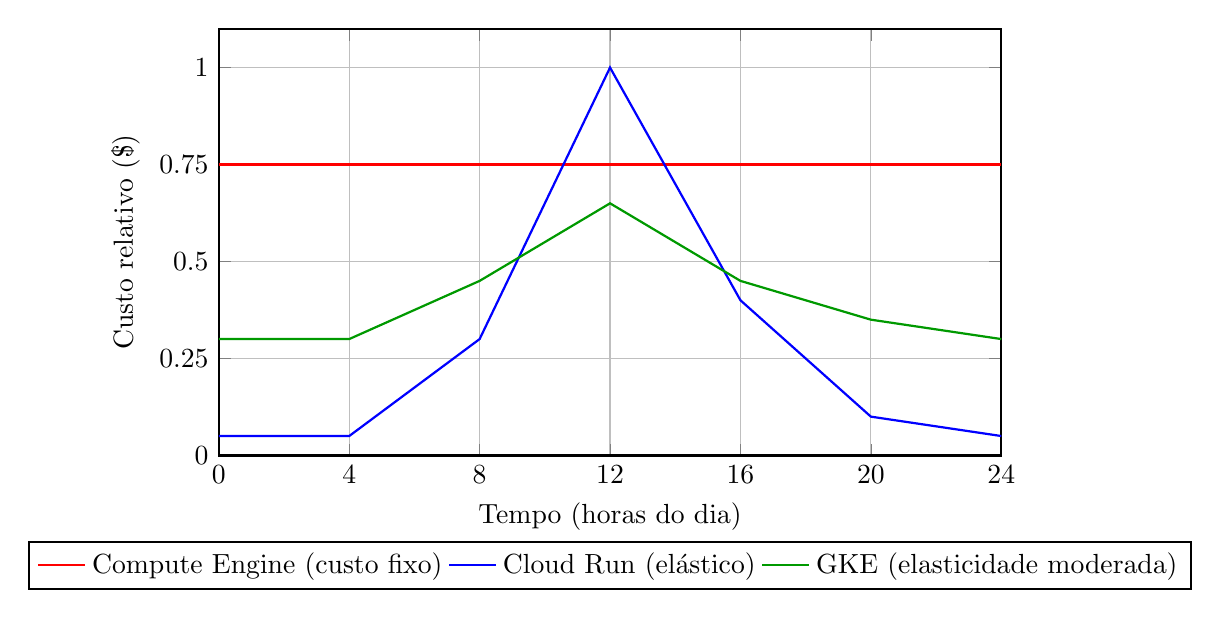
\begin{tikzpicture}
\begin{axis}[
    width=0.95\linewidth,
    height=7cm,
    xlabel={Tempo (horas do dia)},
    ylabel={Custo relativo (\$)},
    xmin=0, xmax=24,
    ymin=0, ymax=1.1,
    xtick={0,4,8,12,16,20,24},
    ytick={0,0.25,0.5,0.75,1.0},
    grid=major,
    legend style={at={(0.5,-0.20)},anchor=north,legend columns=3},
    thick,
]

% Compute Engine (custo estável)
\addplot[red, thick] coordinates {
    (0,0.75) (4,0.75) (8,0.75) (12,0.75) (16,0.75) (20,0.75) (24,0.75)
};
\addlegendentry{Compute Engine (custo fixo)}

% Cloud Run (custo proporcional)
\addplot[blue, thick] coordinates {
    (0,0.05) (4,0.05) (8,0.3) (12,1.0) (16,0.4) (20,0.1) (24,0.05)
};
\addlegendentry{Cloud Run (elástico)}

% GKE (curva intermediária)
\addplot[green!60!black, thick] coordinates {
    (0,0.3) (4,0.3) (8,0.45) (12,0.65) (16,0.45) (20,0.35) (24,0.3)
};
\addlegendentry{GKE (elasticidade moderada)}

\end{axis}
\end{tikzpicture}
\caption{Comparação conceitual do custo relativo ao longo do dia entre Compute Engine, Cloud Run e GKE, assumindo tráfego variável com pico ao meio-dia.}
\label{fig:custo-conceitual}
\end{figure}

A Figura~\ref{fig:custo-conceitual} ilustra conceitualmente o comportamento de custos ao longo do dia para três modelos de execução. Em workloads com picos concentrados — como os observados nos cenários deste TCC — o Cloud Run segue o perfil de tráfego, cobrando mais apenas próximo ao pico e retornando praticamente a zero nas horas ociosas. Já o Compute Engine mantém custo constante, independentemente da demanda. O GKE apresenta comportamento intermediário: embora reduza custos fora do pico, o autoscaler tende a manter nós parcialmente ociosos, especialmente em cargas irregulares ou altamente dinâmicas.
